\subsection{Mock-up dell'applicazione}
    \begin{flushleft}
       
        L'interfaccia utente  ha il compito di “filtrare” la complessità, presentando all'utente un'immagine semplificata del prodotto, e congruente con i compiti che egli deve
        svolgere. Una buona interfaccia non solo nasconde la complessità interna del sistema, ma ne riduce la
        complessità funzionale, mettendo a disposizione dell'utente funzioni di più alto livello, in grado di effettuare compiti
        complessi con un grado di automatismo maggiore. (da "Facile da Usare")\\
        Di seguito verranno presentati i mockup relativi all'applicazione. (Si noti che in questa fase i prototipi dell'interfaccia grafica potrebbero differire da quella che sarà poi la versione finale dell'applicazione.)
        Anche in questo caso abbiamo usato tool molto potenti per la prototipazione delle viste dell'app. Più in particolare, ci siamo avvalsi del tool di design \textbf{Figma}.
        
        \begin{figure}[H]
          \centering
          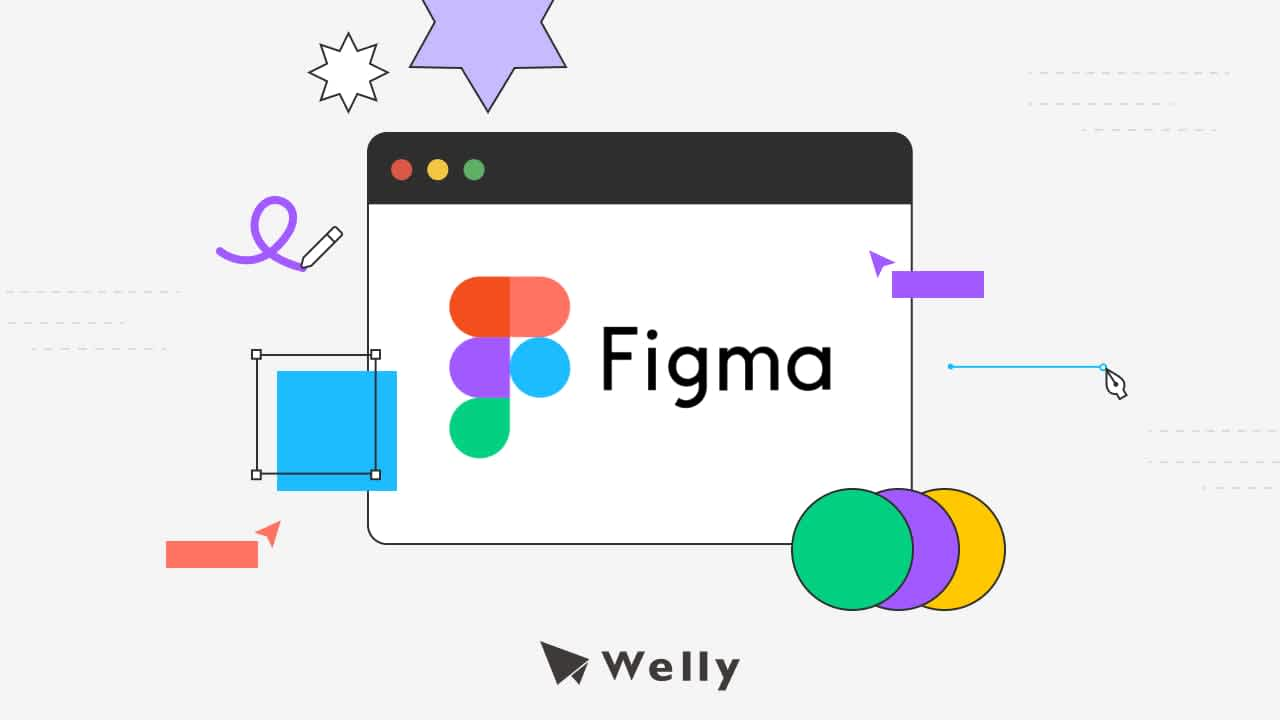
\includegraphics[scale=0.5]{assets/immagini varie/figma.jpg}
          \caption{Tool Figma}\label{fig:figma}
        \end{figure}

        \vspace{2cm}
         \begin{figure}[H]
          \centering
          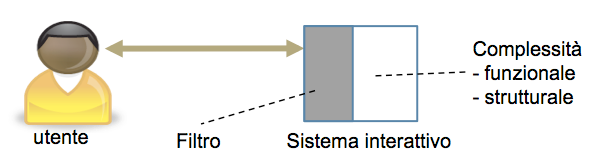
\includegraphics[scale=0.7]{assets/immagini varie/interfaccia utente.png}
          \caption{L'interfaccia Utente}\label{fig:interfaccia utente}
        \end{figure}

    \end{flushleft}

    \newpage

    \subsubsection{Homepage dell'applicazione}
        \begin{figure}[H]
          \centering
          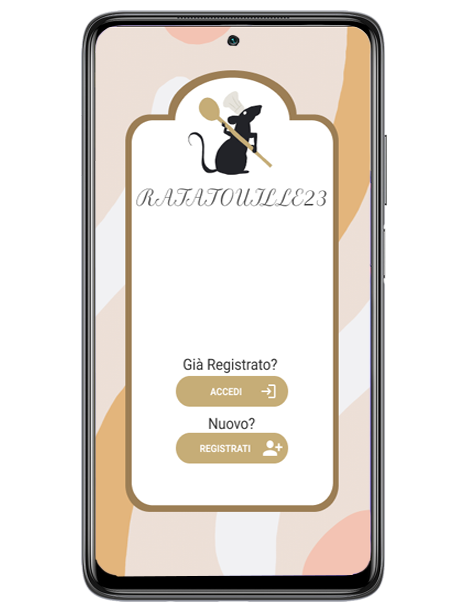
\includegraphics[scale=0.5]{assets/diagrammi/Mockup/Mockup_Homepage.png}
          \caption{\textbf{M01}: Homepage dell'applicazione}\label{fig:Mockup_Homepage}
        \end{figure}

        \newpage

        \begin{flushleft}
            \textbf{ID} \ \Large{ \emph{\textbf{M01}}}\\
        \end{flushleft}

        \textbf{Componenti}:

        \begin{center}
          \begin{tblr}{hlines = {0.9pt}, vlines = {0.9pt}, row{1} = {marroneApp!60}, colspec = {X[c]X[c]X[c]}, width = \textwidth}
            \textbf{Tipo}  &   \textbf{Nome} & \textbf{Funzione} \\
            Bottone        &   ACCEDI        & Quando cliccato porta alla schermata  \emph{\textbf{M02}} \\
            Bottone        &   REGISTRATI   & Quando cliccato porta alla schermata  \emph{\textbf{M03}}  \\
          \end{tblr}
        \end{center}
        
        \newpage

        \subsubsection{Schermata di accesso nel sistema}
            \begin{figure}[H]
                \centering
                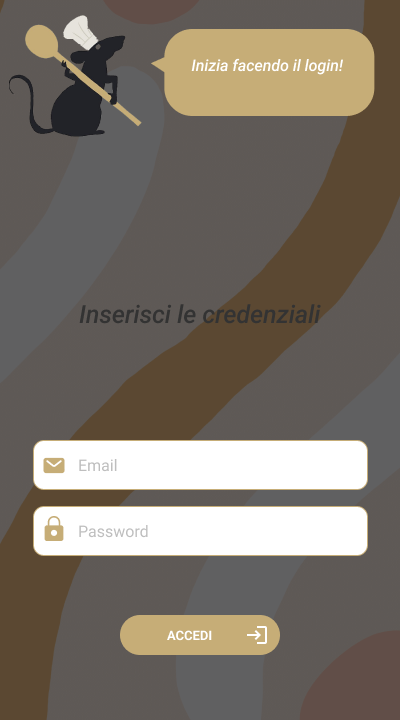
\includegraphics[scale=0.5]{assets/diagrammi/Mockup/Mockup_Accesso.png}
                \caption{\textbf{M02}: Schermata di accesso nel sistema}\label{fig:Mockup_Login}
            \end{figure}
            \begin{flushleft}
                \textbf{ID} \ \Large{ \emph{\textbf{M02}}}\\
            \end{flushleft}

            \textbf{Componenti}:

            \begin{center}
              \begin{tblr}{hlines = {0.9pt}, vlines = {0.9pt}, row{1} = {marroneApp!60}, colspec = {X[c]X[c]X[c]}, width = \textwidth}
                \textbf{Tipo}   &   \textbf{Nome}   &   \textbf{Funzione} \\
                Edit Text       &   EMAIL &   Permette l'inserimento dell'email dell'utente \\
                Edit Text       &   PASSWORD  &  Permette l'inserimento della password dell'utente  \\
                Bottone         &   ENTRA   & Quando cliccato porta alla schermata  \emph{\textbf{M04}} se admin,  \emph{\textbf{M09}} se supervisore,  \emph{\textbf{M11}} se cameriere,  \emph{\textbf{M12}} se account della cucina \\
              \end{tblr}
            \end{center}

        \newpage
        \subsubsection{Schermata di registrazione nel sistema}
        \begin{figure}[H]
          \centering
          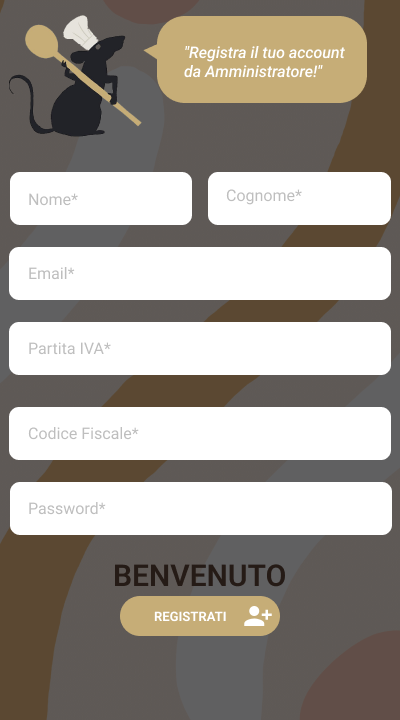
\includegraphics[scale=0.25]{assets/diagrammi/Mockup/Mockup_Register.png}
          \caption{\textbf{M03}: Schermata di registrazione nel sistema}\label{fig:Mockup_Register}
        \end{figure}

        \begin{flushleft}
          \textbf{ID} \ \Large{ \emph{\textbf{M03}}}\\
          \large{ \emph{Nota}: la schermata di registrazione è valida solo per gli admin proprietari dei ristoranti, in quanto sono poi loro a registrare i dipendenti.}\\
        \end{flushleft}

        \textbf{Componenti}:

            \begin{center}
              \begin{longtblr}{hlines = {0.9pt}, vlines = {0.9pt}, row{1} = {marroneApp!60}, colspec = {X[c]X[c]X[c]}, width = \textwidth, rowhead=1}
                \textbf{Tipo}   &   \textbf{Nome}   &   \textbf{Funzione} \\
                Edit Text    &   NOME    &   Permette di inserire il nome dell'admin \\
                Edit Text & COGNOME   &  Permette di inserire il cognome dell'admin \\
                Edit Text    &   PASSWORD    &   Permette di inserire una password per l'admin \\
                Edit Text    &   EMAIL   &   Permette di inserire l'email dell'admin \\
                Edit Text    & CODICE FISCALE    & Permette di inserire il codice fiscale dell'admin \\
                Edit Text    &   P.IVA   & Permette di inserire la partita IVA dell'admin \\
                Bottone &   REGISTRATI  & Quando cliccato riporta alla schermata  \emph{\textbf{M01}} per permettere l'accesso \\
              \end{longtblr}
            \end{center}
        \newpage
        \subsubsection{Schermata home per gli admin}
        \begin{figure}[H]
            \centering
            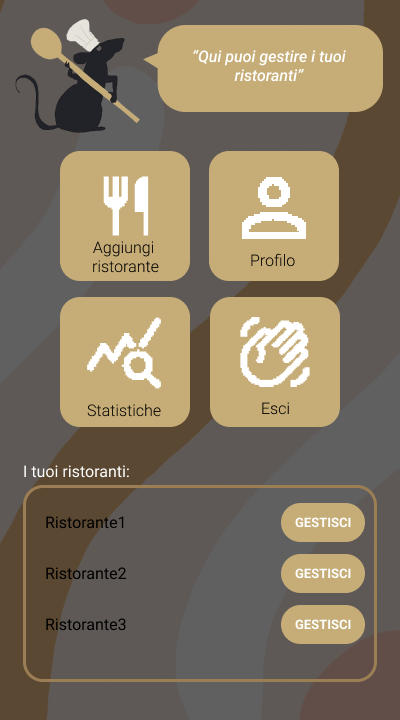
\includegraphics[scale=0.35]{assets/diagrammi/Mockup/Mockup_AdminDash.png}
            \caption{\textbf{M04}: Schermata home per gli admin}\label{fig:Mockup_AdminDashboard}
        \end{figure}
        \begin{flushleft}
            \textbf{ID} \ \Large{ \emph{\textbf{M04}}} \\
        \end{flushleft}
        \textbf{Componenti}:

            \begin{center}
                \begin{longtblr}{hlines = {0.9pt}, vlines = {0.9pt}, row{1} = {marroneApp!60}, colspec = {X[c]X[c]X[c]}, width = \textwidth, rowhead=1}
                \textbf{Tipo}   &   \textbf{Nome}   &   \textbf{Funzione} \\
                ScrollView &   I TUOI RISTORANTI    &   Visualizza ed eventualmente permette la modifica dei ristoranti registrati\\
                Bottone    &   AGGIUNGI RISTORANTE  &   Quando cliccato porta alla schermata  \emph{\textbf{M05}} \\
                Bottone    &   MODIFICA   &   Quando cliccato porta alla schermata  \emph{\textbf{M06}} \\
                Bottone    &   PROFILO    &   Quando cliccato porta alla schermata  \emph{\textbf{M13}} \\
                Bottone    &   ESCI       &   Quando cliccato mostra la schermata  \emph{\textbf{M10}} \\
                Bottone    &   STATISTICHE &  Quando cliccato porta alla schermata  \emph{\textbf{M20}} \\
                \end{longtblr}
            \end{center}
        \newpage

        \subsubsection{Schermata di registrazione di un nuovo ristorante}
        \begin{figure}[H]
            \centering
            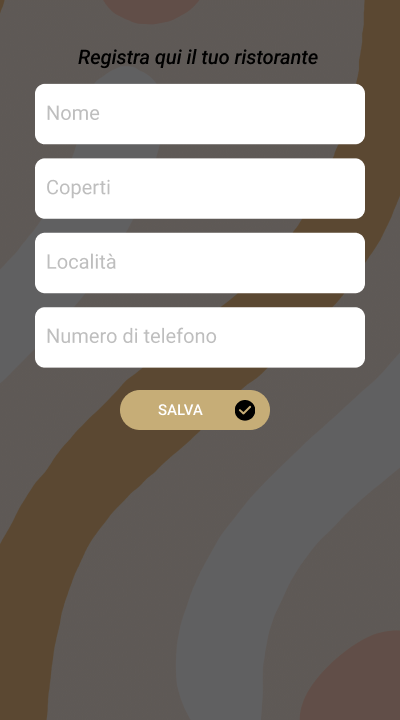
\includegraphics[scale=0.35]{assets/diagrammi/Mockup/Mockup_SaveResturant.png}
            \caption{\textbf{M05}: Schermata di registrazione di un nuovo ristorante}\label{fig:Mockup_AddResturant}
        \end{figure}
        \begin{flushleft}
            \textbf{ID} \ \Large{ \emph{\textbf{M05}}}
        \end{flushleft}
        \textbf{Componenti}:

        \begin{center}
          \begin{tblr}{hlines = {0.9pt}, vlines = {0.9pt}, row{1} = {marroneApp!60}, colspec = {X[c]X[c]X[c]}, width = \textwidth}
            \textbf{Tipo}  &   \textbf{Nome}  & \textbf{Funzione} \\
            Edit Text      &   NOME           & Permette di inserire il nome del nuovo ristorante\\
            Edit Text      &   LOCALITA'      & Permette di inserire la località del nuovo ristorante\\
            Edit Text      &   COPERTI        & Permette di inserire il n° dei coperti del nuovo ristorante\\
            Edit Text      &   NUMERO DI TELEFONO & Permette di inserire il contatto telefonico del ristorante \\
            Bottone        &   SALVA          & Quando cliccato salva il nuovo ristorante nel database e torna alla schermata  \emph{\textbf{M04}} \\
          \end{tblr}
        \end{center}
        \newpage
        \subsubsection{Schermata di modifica di un ristorante}
        \begin{figure}[H]
            \centering
            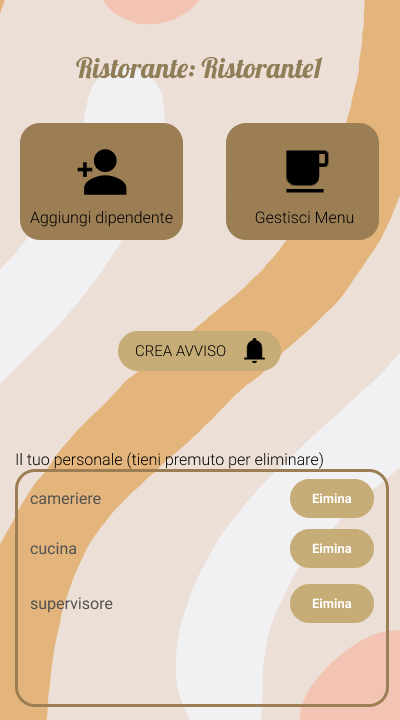
\includegraphics[scale=0.4]{assets/diagrammi/Mockup/Mockup_ResturantDash.png}
            \caption{\textbf{M06}: Schermata di modifica di un ristorante}\label{fig:Mockup_ResturantManager}
        \end{figure}
        \begin{flushleft}
            \textbf{ID} \ \Large{ \emph{\textbf{M06}}}
        \end{flushleft}

        \textbf{Componenti}:

          \begin{center}
            \begin{tblr}{hlines = {0.9pt}, vlines = {0.9pt}, row{1} = {marroneApp!60}, colspec = {X[c]X[c]X[c]}, width = \textwidth}
              \textbf{Tipo}  &   \textbf{Nome}  & \textbf{Funzione} \\
              Bottone   &   AGGIUNGI DIPENDENTE &   Quando cliccato porta alla schermata  \emph{\textbf{M07}}\\
              Bottone   &   GESTISCI MENU &   Quando cliccato porta alla schermata  \emph{\textbf{M08}}\\
              ScrollView  & IL TUO PERSONALE  & Mostra il personale che lavora nel ristorante, dove se si tiene premuto il bottone  \emph{Elimina} viene eliminato l'account del dipendente scelto dal ristorante \\
              Bottone   &   CREA AVVISO   &   Quando cliccato mostra la schermata  \emph{\textbf{M17}} \\  
            \end{tblr}
          \end{center}

        \newpage

        \subsubsection{Schermata di registrazione di un nuovo dipendente}
        \begin{figure}[H]
            \centering
            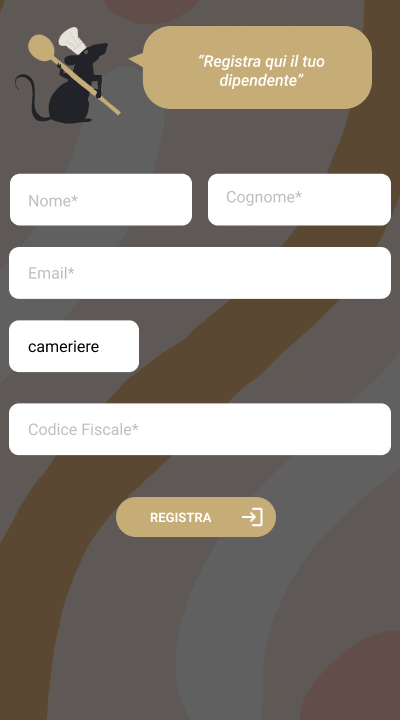
\includegraphics[scale=0.35]{assets/diagrammi/Mockup/Mockup_SaveWorker.png}
            \caption{\textbf{M07}: Schermata di registrazione di un nuovo dipendente}\label{fig:Mockup_SaveWaiter}
        \end{figure}
        \begin{flushleft}
            \textbf{ID} \ \Large{ \emph{\textbf{M07}}}
        \end{flushleft}
        \textbf{Componenti}:

        \begin{center}
          \begin{tblr}{hlines = {0.9pt}, vlines = {0.9pt}, row{1} = {marroneApp!60}, colspec = {X[c]X[c]X[c]}, width = \textwidth}
            \textbf{Tipo}   &   \textbf{Nome}   &   \textbf{Funzione} \\
            Edit Text   &   NOME    &   Permette di inserire il nome del nuovo dipendente\\
            Edit Text   &   COGNOME   &   Permette di inserire il cognome del nuovo dipendente\\
            Edit Text   &   EMAIL   & Permette di inserire l'email del nuovo dipendente\\
            Edit Text   &   CODICE FISCALE    &   Permette di inserire il codice fiscale del nuovo dipendente \\
            Spinner &   {cameriere\\ (default)}    &   Permette di inserire il ruolo del nuovo dipendente \\
            Bottone &   REGISTRA    &   Quando cliccato, se tutti i dati sono corretti, riporta alla schermata  \emph{\textbf{M04}} registrando il nuovo dipendente \\
          \end{tblr}
        \end{center}

        \newpage

        \subsubsection{Schermata di gestione del menù}
        \begin{figure}[H]
            \centering
            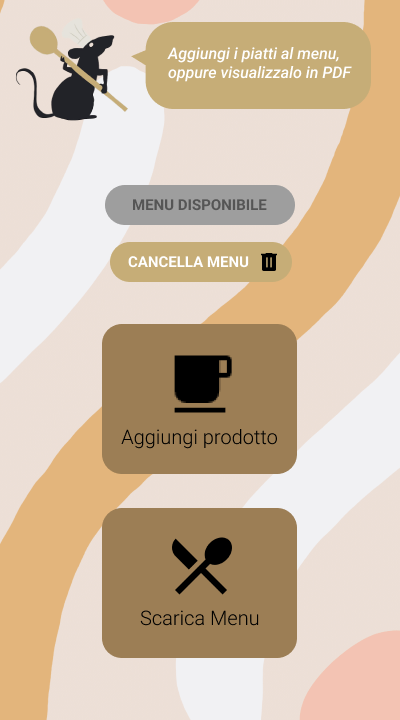
\includegraphics[scale=0.35]{assets/diagrammi/Mockup/Mockup_MenuManager.png}
            \caption{\textbf{M08}: Schermata di gestione del menù}\label{fig:Mockup_MenuManager}
        \end{figure}
        \begin{flushleft}
            \textbf{ID} \ \Large{ \emph{\textbf{M08}}}
        \end{flushleft}
        \textbf{Componenti}:

        \begin{center}
          \begin{tblr}{hlines = {0.9pt}, vlines = {0.9pt}, row{1} = {marroneApp!60}, colspec = {X[c]X[c]X[c]}, width = \textwidth}
            \textbf{Tipo}   &   \textbf{Nome}   &   \textbf{Funzione} \\
            Bottone   &   AGGIUNGI PRODOTTO    &   Quando cliccato porta alla schermata  \emph{\textbf{M18}}\\
            Edit Text   &   SCARICA MENU   &   Permette di generare il menù e salvarlo sul dispositivo in formato PDF\\
            Bottone   &   CREA MENU       &   Quando cliccato permette di creare un menu (se non è gia stato creato) \\
            Bottone   &   CANCELLA MENU   &   Permette di cancellare il menu del ristorante (se esistente) \\
          \end{tblr}
        \end{center}

        \newpage

        \subsubsection{Schermata home per i supervisori}
          \begin{figure}[H]
              \centering
              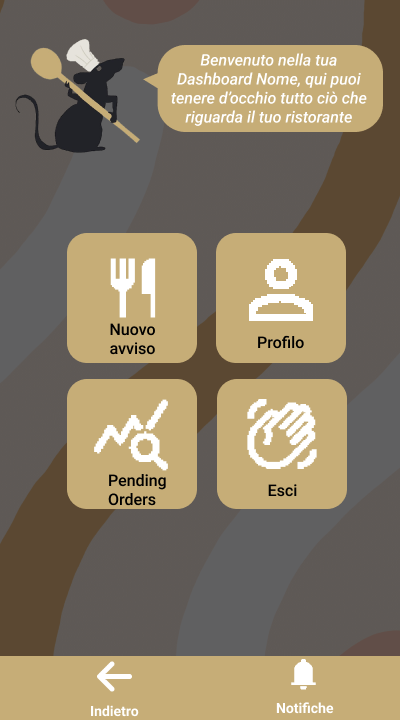
\includegraphics[scale=0.35]{assets/diagrammi/Mockup/Mockup_HypervisorDash.png}
              \caption*{\textbf{M09}: Schermata home dei supervisori}\label{fig:Mockup_HypervisorDash}
          \end{figure}

          \begin{flushleft}
              \textbf{ID}   \ \Large{ \emph{\textbf{M09}}}
          \end{flushleft}

          \textbf{Componenti}:

          \begin{center}
              \begin{tblr}{hlines = {0.9pt}, vlines = {0.9pt}, row{1} = {marroneApp!60}, colspec = {X[c]X[c]X[c]}, width = \textwidth}
                \textbf{Tipo}   &   \textbf{Nome}   &   \textbf{Funzione} \\
                Bottone   &   PROFILO               &   Quando cliccato porta alla schermata  \emph{\textbf{M13}}  \\
                Bottone   &   NUOVO AVVISO          &   Quando cliccato porta alla schermata  \emph{\textbf{M21}}  \\ 
                Bottone   &   PENDING ORDERS        &   Quando cliccato porta alla schermata  \emph{\textbf{M12}}  \\ 
                Bottone   &   ESCI                  &   Quando cliccato porta alla schermata  \emph{\textbf{M10}}  \\
                Bottom Navigation Bar & BARRA NAVIGAZIONE   &   Permette di visualizzare le notifiche cliccando su  \emph{Notifiche} che porterà alla schermata  \emph{\textbf{M21}} e di tornare indietro cliccando su  \emph{Indietro} \\
              \end{tblr}
          \end{center}

        \newpage

        \subsubsection{Schermata di conferma di uscita}
          \begin{figure}[H]
            \centering
            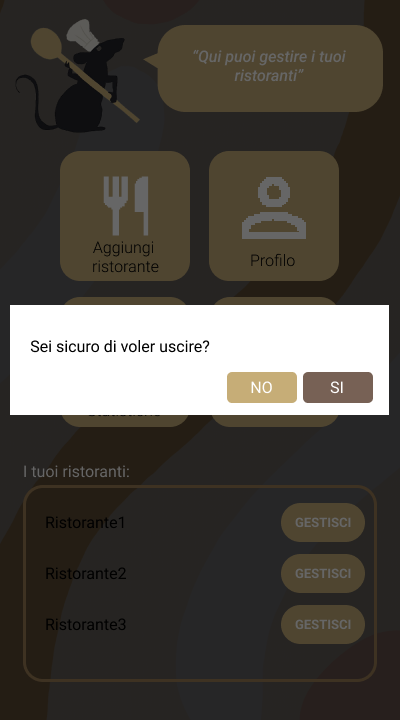
\includegraphics[scale=0.5]{assets/diagrammi/Mockup/Mockup_ExitDialog.png}
            \caption*{\textbf{M10}: Schermata di conferma logout}\label{fig:Mockup_ExitDialog}
          \end{figure}

          \begin{flushleft}
            \textbf{ID}   \ \Large{ \emph{\textbf{M10}}}
          \end{flushleft}

          \textbf{Componenti}:

          \begin{center}
            \begin{tblr}{hlines = {0.9pt}, vlines = {0.9pt}, row{1} = {marroneApp!60}, colspec = {X[c]X[c]X[c]}, width = \textwidth}
              \textbf{Tipo}   &   \textbf{Nome}   &   \textbf{Funzione} \\
              Bottone         &   SI      &   Quando cliccato porta alla schermata  \emph{\textbf{M02}} \\
              Bottone         &   NO      &   Quando cliccato resta nella schermata corrente \\
            \end{tblr}
          \end{center}
        
        \newpage

        \subsubsection{Schermata home per i camerieri}
          \begin{figure}[H]
            \centering
            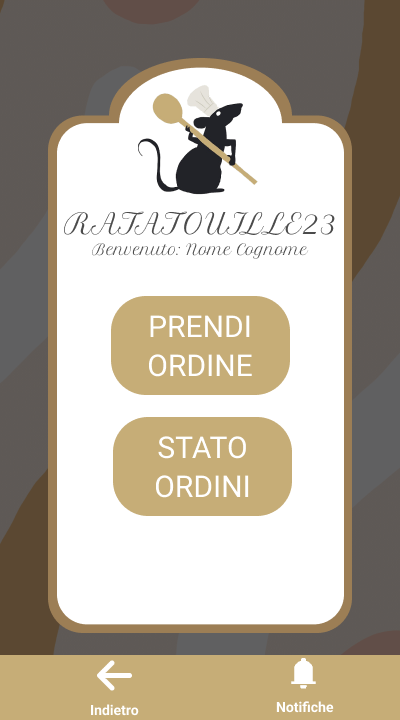
\includegraphics[scale=0.5]{assets/diagrammi/Mockup/Mockup_WaiterDash.png}
            \caption*{\textbf{M11}: Schermata home per i camerieri}
            \label{fig:Mockup_WaiterDash}
          \end{figure}

          \begin{flushleft}
            \textbf{ID}   \ \Large{ \emph{\textbf{M11}}}
          \end{flushleft}

          \textbf{Componenti}:
          
          \begin{center}
            \begin{tblr}{hlines = {0.9pt}, vlines = {0.9pt}, row{1} = {marroneApp!60}, colspec = {X[c]X[c]X[c]}, width = \textwidth}
              \textbf{Tipo}   &   \textbf{Nome}   &   \textbf{Funzione} \\
              Bottone     &   NUOVO ORDINE    &   Quando cliccato porta alla schermata  \emph{\textbf{M19}} \\
              Bottone     &   STATO ORDINE    &   Quando cliccato porta alla schermata  \emph{\textbf{M12}} \\
              Bottom Navigation Bar & BARRA NAVIGAZIONE   &   Permette di visualizzare le notifiche cliccando su  \emph{Notifiche} che porterà alla schermata  \emph{\textbf{M21}} e di tornare indietro cliccando su  \emph{Indietro} \\
            \end{tblr}
          \end{center}

        \newpage

        \subsubsection{Schermata di visualizzazione dello stato degli ordini}

          \begin{figure}[H]
            \centering
            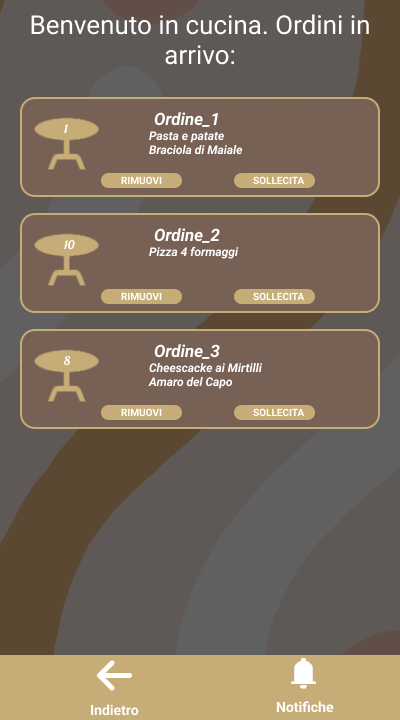
\includegraphics[scale=0.5]{assets/diagrammi/Mockup/Mockup_OrderStatus.png}
            \caption*{\textbf{M12}: Schermata home per i camerieri}
            \label{fig:Mockup_OrderStatus}
          \end{figure}

            \begin{flushleft}
              \textbf{ID}   \ \Large{ \emph{\textbf{M12}}}
            \end{flushleft}
  
            \textbf{Componenti}:
            
            \begin{center}
              \begin{tblr}{hlines = {0.9pt}, vlines = {0.9pt}, row{1} = {marroneApp!60}, colspec = {X[c]X[c]X[c]}, width = \textwidth}
                \textbf{Tipo}   &   \textbf{Nome}   &   \textbf{Funzione} \\
                RecyclerView     &  ORDINI    &   Permette di visualizzare la lista degli ordini, dove per i camerieri vi è la possibilità di sollecitare la cucina su un ordine e per la cucina di evaderlo eliminandolo  \\
                Bottom Navigation Bar & BARRA NAVIGAZIONE   &   Permette di visualizzare le notifiche cliccando su  \emph{Notifiche} che porterà alla schermata  \emph{\textbf{M21}} e di tornare indietro cliccando su  \emph{Indietro} \\ 
              \end{tblr}
            \end{center}

            \newpage

            \subsubsection{Schermata di visualizzazione del profilo}
              \begin{figure}[H]
                \centering
                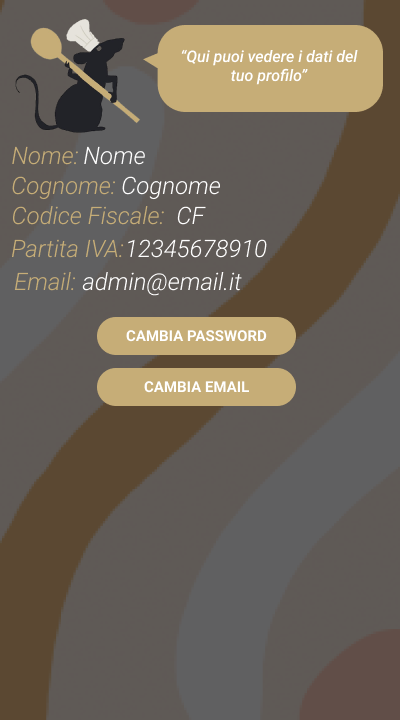
\includegraphics[scale=0.5]{assets/diagrammi/Mockup/Mockup_Profile.png}
                \caption*{\textbf{M13}: Schermata visualizzazione profilo}\label{fig:Mockup_Profile}
              \end{figure}
    
              \begin{flushleft}
                \textbf{ID}   \ \Large{ \emph{\textbf{M13}}}
              \end{flushleft}
    
              \textbf{Componenti}:
              
              \begin{center}
                \begin{tblr}{hlines = {0.9pt}, vlines = {0.9pt}, row{1} = {marroneApp!60}, colspec = {X[c]X[c]X[c]}, width = \textwidth}
                  \textbf{Tipo}   &   \textbf{Nome}   &   \textbf{Funzione} \\
                  Bottone     &   CAMBIA PASSWORD   &   Quando cliccato mostra la schermata  \emph{\textbf{M14}}  \\
                  Bottone     &   CAMBIA EMAIL   &   Quando cliccato mostra la schermata  \emph{\textbf{M15}}  \\    
                \end{tblr}
              \end{center}

              \newpage

              \subsubsection{Schermata di cambio password per gli admin}
                \begin{figure}[H]
                  \centering
                  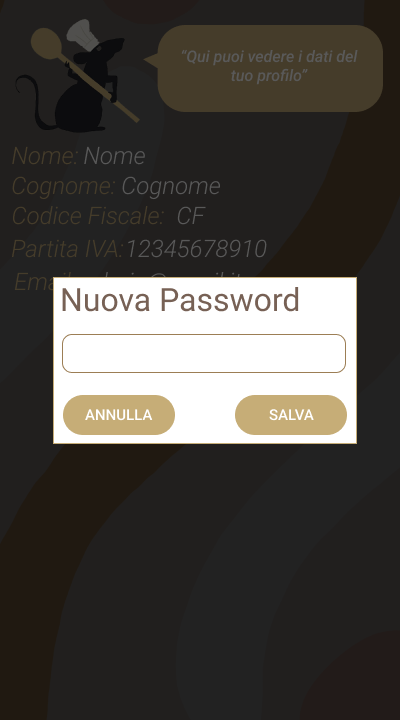
\includegraphics[scale=0.5]{assets/diagrammi/Mockup/Mockup_AdminChangePass.png}
                  \caption*{\textbf{M14}: Schermata cambio password admin}\label{fig:Mockup_AdminChangePass}
                \end{figure}
      
                \begin{flushleft}
                  \textbf{ID}   \ \Large{ \emph{\textbf{M14}}}
                \end{flushleft}
      
                \textbf{Componenti}:
                
                \begin{center}
                  \begin{tblr}{hlines = {0.9pt}, vlines = {0.9pt}, row{1} = {marroneApp!60}, colspec = {X[c]X[c]X[c]}, width = \textwidth}
                    \textbf{Tipo}   &   \textbf{Nome}   &   \textbf{Funzione} \\
                    Edit Text     &   NUOVA PASSWORD    &   Permette di inserire la nuova password per l'account dell'admin   \\
                    Bottone     &   ANNULLA   &   Quando cliccato torna alla schermata  \emph{\textbf{M13}} senza effettuare modifiche  \\
                    Bottone     &   SALVA   &   Quando cliccato torna alla schermata  \emph{\textbf{M13}} modificando la password dell'account  \\
                  \end{tblr}
                \end{center}

                \newpage

                \subsubsection{Schermata di cambio email per gli admin}
                  \begin{figure}[H]
                    \centering
                    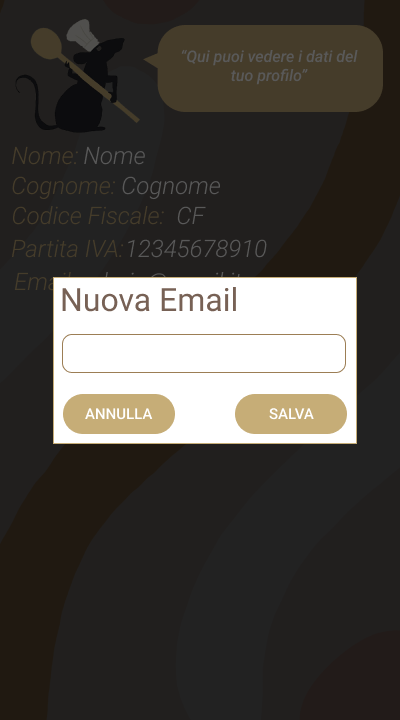
\includegraphics[scale=0.5]{assets/diagrammi/Mockup/Mockup_AdminChangeMail.png}
                    \caption*{\textbf{M15}: Schermata cambio email admin}\label{fig:Mockup_AdminChangeMail}
                  \end{figure}
        
                  \begin{flushleft}
                    \textbf{ID}   \ \Large{ \emph{\textbf{M15}}}
                  \end{flushleft}
        
                  \textbf{Componenti}:
                  
                  \begin{center}
                    \begin{tblr}{hlines = {0.9pt}, vlines = {0.9pt}, row{1} = {marroneApp!60}, colspec = {X[c]X[c]X[c]}, width = \textwidth}
                      \textbf{Tipo}   &   \textbf{Nome}   &   \textbf{Funzione} \\
                      Edit Text   &   NUOVA EMAIL   &   Permette di inserire la nuova email per l'account dell'admin  \\
                      Bottone     &   ANNULLA   &   Quando cliccato torna alla schermata  \emph{\textbf{M13}} senza effettuare modifiche  \\
                      Bottone     &   SALVA   &   Quando cliccato torna alla schermata  \emph{\textbf{M13}} modificando l'email dell'account  \\
                    \end{tblr}
                  \end{center}

                \newpage

                \subsubsection{Schermata di cambio password per i dipendenti al primo accesso}
                    \begin{figure}[H]
                      \centering
                      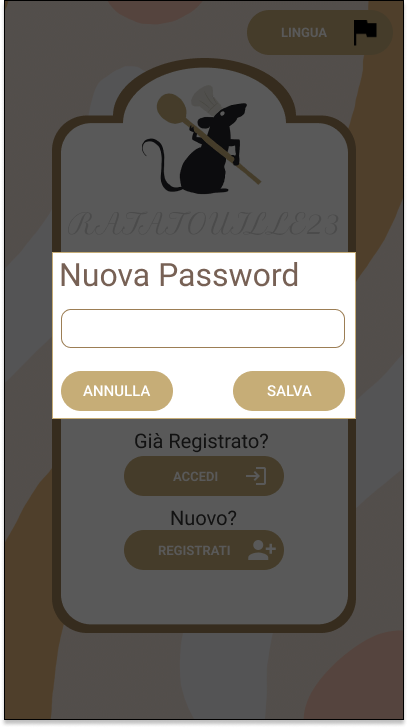
\includegraphics[scale=0.35]{assets/diagrammi/Mockup/Mockup_WorkerChangePass.png}
                      \caption*{\textbf{M16}: Schermata cambio password dipendenti}\label{fig:Mockup_WorkerChangePass}
                    \end{figure}
          
                    \begin{flushleft}
                      \textbf{ID}   \ \Large{ \emph{\textbf{M16}}}
                    \end{flushleft}
          
                    \textbf{Componenti}:
                    
                    \begin{center}
                      \begin{tblr}{hlines = {0.9pt}, vlines = {0.9pt}, row{1} = {marroneApp!60}, colspec = {X[c]X[c]X[c]}, width = \textwidth}
                        \textbf{Tipo}   &   \textbf{Nome}   &   \textbf{Funzione} \\
                        Edit Text   &   NUOVA PASSWORD   &   Permette di inserire la nuova password per l'account del dipendente  \\
                        Bottone     &   ANNULLA   &   Quando cliccato torna alla schermata  \emph{\textbf{M02}} senza effettuare modifiche  \\
                        Bottone     &   SALVA   &   Quando cliccato porta alla schermata  \emph{\textbf{M09}} se è supervisore,  \emph{\textbf{M11}} se è cameriere,  \emph{\textbf{M12}} se è un account di cucina, modificando l'email dell'account  \\
                      \end{tblr}
                    \end{center}

                  \newpage

                  \subsubsection{Schermata di creazione degli avvisi}
                      \begin{figure}[H]
                        \centering
                        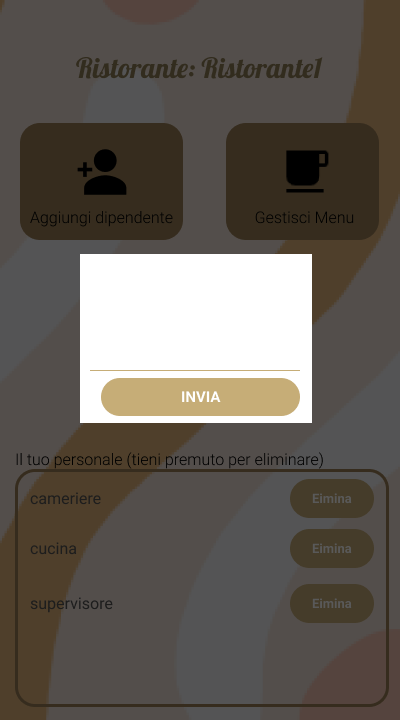
\includegraphics[scale=0.5]{assets/diagrammi/Mockup/Mockup_SaveAdv.png}
                        \caption*{\textbf{M17}: Schermata creazione avvisi}\label{fig:Mockup_SaveAdv}
                      \end{figure}
            
                      \begin{flushleft}
                        \textbf{ID}   \ \Large{ \emph{\textbf{M17}}}
                      \end{flushleft}
            
                      \textbf{Componenti}:

                      \begin{center}
                        \begin{tblr}{hlines = {0.9pt}, vlines = {0.9pt}, row{1} = {marroneApp!60}, colspec = {X[c]X[c]X[c]}, width = \textwidth}
                          \textbf{Tipo}   &   \textbf{Nome}   &   \textbf{Funzione} \\
                          Edit Text     &   AVVISO    &   Permette di inserire il testo dell'avviso \\
                          Bottone       &   INVIA      &   Quando cliccato torna alla schermata  \emph{\textbf{M06}} inviando l'avviso \\
                        \end{tblr}
                      \end{center}

                    \newpage

                    \subsubsection{Schermata di aggiunta piatti al menù}
                        \begin{figure}[H]
                          \centering
                          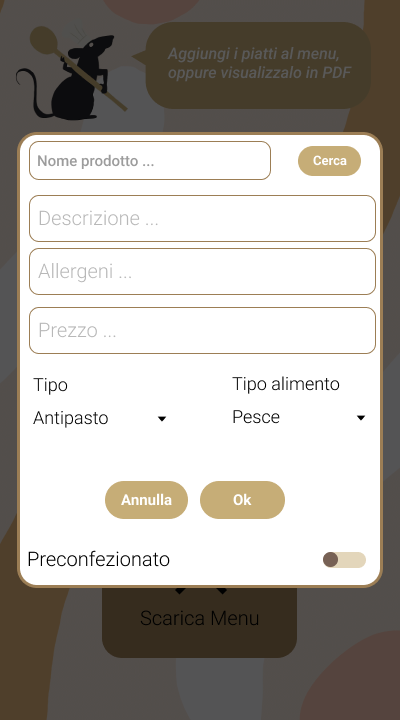
\includegraphics[scale=0.5]{assets/diagrammi/Mockup/Mockup_AddPlate.png}
                          \caption*{\textbf{M18}: Schermata aggiunta piatti al menù}\label{fig:Mockup_AddPlate}
                        \end{figure}
              
                        \begin{flushleft}
                          \textbf{ID}   \ \Large{ \emph{\textbf{M18}}}
                        \end{flushleft}
              
                        \textbf{Componenti}:
                        
                        \begin{center}
                          \begin{longtblr}{hlines = {0.9pt}, vlines = {0.9pt}, row{1} = {marroneApp!60}, colspec = {X[c]X[c]X[c]}, width = \textwidth, rowhead=1}
                            \textbf{Tipo}   &   \textbf{Nome}   &   \textbf{Funzione} \\
                            EditText        &   NOME PRODOTTO   &   Permette di inserire il titolo del prodotto da inserire \\
                            EditText        &   DESCRIZIONE     &   Permette di inserire la descrizione del prodotto da Inserire  \\
                            EditText        &   ALLERGENI       &   Permette di inserire gli allergeni contenuti nel prodotto \\
                            EditText        &   PREZZO          &   Permette di inserire il prezzo del prodotto \\
                            Spinner         &   TIPO            &   Permette di inserire il tipo di portata (antipasto, primo, ...) \\
                            Spinner         &   TIPO DI ALIMENTO &  Permette di inserire il tipo di alimento (carne, pesce, ...)  \\
                            Bottone         &   CERCA           &   Quando cliccato, ricerca il prodotto scritto nel database di OpenFoodFacts  \\
                            Bottone         &   OK              &   Quando cliccato, ritorna alla schermata  \emph{\textbf{M08}} salvando nel menu il prodotto \\
                            Bottone         &   ANNULLA         &   Quando cliccate, ritorna alla schermata  \emph{\textbf{M08}} senza salvare il prodotto \\  
                            Selettore       &   PRECONFEZIONATO &   Se selezionato, indica che l'oggetto è di tipo preconfezionato(bibita, ...) \\
                          \end{longtblr}
                        \end{center}

                      \newpage

                    \subsubsection{Schermata di aggiunta ordini}
                          \begin{figure}[H]
                            \centering
                            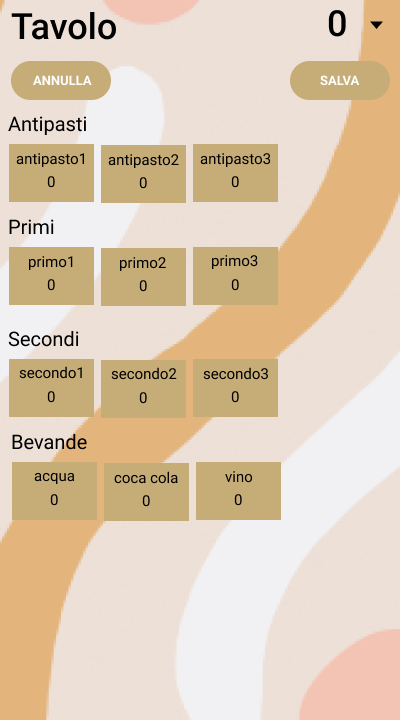
\includegraphics[scale=0.4]{assets/diagrammi/Mockup/Mockup_AddOrder.png}
                            \caption*{\textbf{M19}: Schermata aggiunta ordini}\label{fig:Mockup_AddOrder}
                          \end{figure}
                
                          \begin{flushleft}
                            \textbf{ID}   \ \Large{ \emph{\textbf{M19}}}
                          \end{flushleft}
                
                          \textbf{Componenti}:
                          
                          \begin{center}
                            \begin{tblr}{hlines = {0.9pt}, vlines = {0.9pt}, row{1} = {marroneApp!60}, colspec = {X[c]X[c]X[c]}, width = \textwidth}
                              \textbf{Tipo}   &   \textbf{Nome}   &   \textbf{Funzione} \\
                              ScrollView      &   PIATTI    &   Visualizza la lista dei piatti del menù del ristorante, dove ogni piatto si può cliccare per aggiungerlo all'ordine \\
                              Bottone         &   SALVA     &   Quando cliccato porta alla schermata  \emph{\textbf{M11}} inviando l'ordine \\
                              Bottone         &   INDIETRO  &   Quando cliccato porta alla schermata  \emph{\textbf{M11}} senza effettuare nessuna azione \\
                            \end{tblr}
                          \end{center}
                    
                    \newpage

                    \subsubsection{Schermata di visualizzazione delle statistiche}
                      \begin{figure}[H]
                        \centering
                        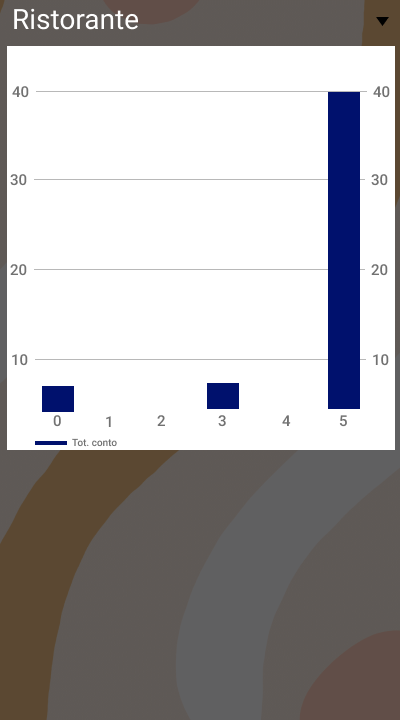
\includegraphics[scale=0.5]{assets/diagrammi/Mockup/Mockup_Statistics.png}
                        \caption*{\textbf{M20}: Schermata visualizzazione statistiche}\label{fig:Mockup_Statistics}
                      \end{figure}

                      \begin{flushleft}
                        \textbf{ID}   \ \Large{ \emph{\textbf{M20}}}
                      \end{flushleft}

                      \textbf{Componenti}:

                      \begin{center}
                        \begin{longtblr}{hlines = {0.9pt}, vlines = {0.9pt}, row{1} = {marroneApp!60}, colspec = {X[c]X[c]X[c]}, width = \textwidth, rowhead=1}
                          \textbf{Tipo}   &   \textbf{Nome}   &   \textbf{Funzione} \\
                          Spinner         &   RISTORANTE             &   Permette di selezionare il ristorante di cui si vogliono visualizzazione le statistiche \\
                          ScrollView      &   GRAFICI STATISTICHE    &   Permette di visualizzare i grafici relativi alle statistiche di  \emph{Ristorante} \\
                        \end{longtblr}
                      \end{center}
                    
                    \newpage

                    \subsubsection{Schermata di visualizzazione delle notifiche}
                      \begin{figure}[H]
                        \centering
                        
\includegraphics[scale=0.4]{assets/diagrammi/Mockup/Mockup_Notifications.png}
                        \caption*{\textbf{M21}: Schermata visualizzazione notifiche}\label{fig:Mockup_Notifications}
                      \end{figure}

                      \begin{flushleft}
                        \textbf{ID}   \ \Large{ \emph{\textbf{M21}}}
                      \end{flushleft}

                      \textbf{Componenti}:

                      \begin{center}
                        \begin{longtblr}{hlines = {0.9pt}, vlines = {0.9pt}, row{1} = {marroneApp!60}, colspec = {X[c]X[c]X[c]}, width = \textwidth, rowhead=1}
                          \textbf{Tipo}   &   \textbf{Nome}   &   \textbf{Funzione} \\
                          ScrollView      &   NOTIFICHE    &   Permette di visualizzare le varie notifiche ricevute dal proprio ristorante, inviate dall'admin o dal supervisore, contenenti: 
                                                                \emph{Nome}, 
                                                                \emph{Data e ora},
                                                                \emph{Messaggio}, 
                                                               che tramite swipe verso sinistra vengono segnati come letti ed eliminati dalla schermata \\
                        \end{longtblr}
                      \end{center}